\documentclass[12pt]{article}
\setlength{\oddsidemargin}{0in}
\setlength{\evensidemargin}{0in}
\setlength{\textwidth}{6.5in}
\setlength{\parindent}{0in}
\setlength{\parskip}{\baselineskip}

\usepackage{amsmath,amsfonts,amssymb,graphicx, hyperref, float}

\begin{document}

IBEHS 4A03 \hfill Assignment \#2\\
Baoze Lin, Hady Ibrahim

\hrulefill

% Custom numbering for subparts (e.g., 2.1, 2.2)
\renewcommand{\theenumii}{\arabic{enumi}.\arabic{enumii}}

\begin{enumerate}
\item Question 1
  \begin{enumerate}
    % ANSWER TO 1.1
    \item
    The pole-zero maps for \( Y_1(s) \) and \( Y_2(s) \) help us see system stability. 

    - The left plot shows the pole-zero locations for \( Y_1(s) \), which has poles in the left half-plane, indicating a stable system. The poles are: $s=0, -2, -3$. \\
    - The right plot for \( Y_2(s) \) shows at minimum 1 pole in the right half-plane, meaning the system is unstable and will have an exponentially growing response. The poles are: $s=0, 2, 1+2i, 1-2i$.

    \begin{figure}[H]
      \centering
      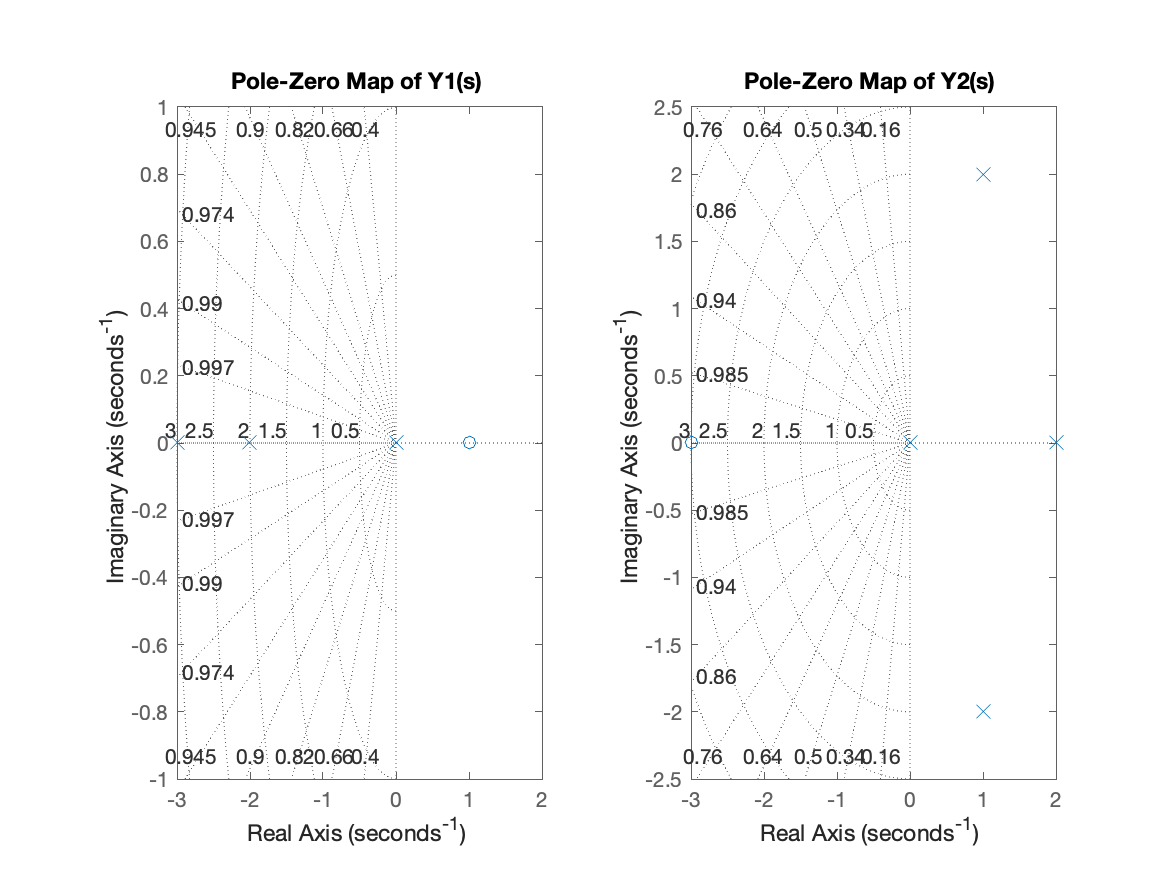
\includegraphics[width=0.8\textwidth]{Figures/figure1-1.png}
      \caption{Pole-Zero Maps for \( Y_1(s) \) and \( Y_2(s) \)}
      \label{fig:figure11} 
    \end{figure}

    \pagebreak
    % ANSWER TO 1.2
    \item
    The Final Value Theorem was used to determine the steady-state values (via hand calculation and using limit() in Matlab):

    \[
    \lim_{t \to \infty} y_1(t) = \lim_{s \to 0} s Y_1(s) = -\frac{1}{6}
    \]

    \[
    \lim_{t \to \infty} y_2(t) = \lim_{s \to 0} s Y_2(s) = -\frac{3}{10}
    \]

    \begin{figure}[H]
      \centering
      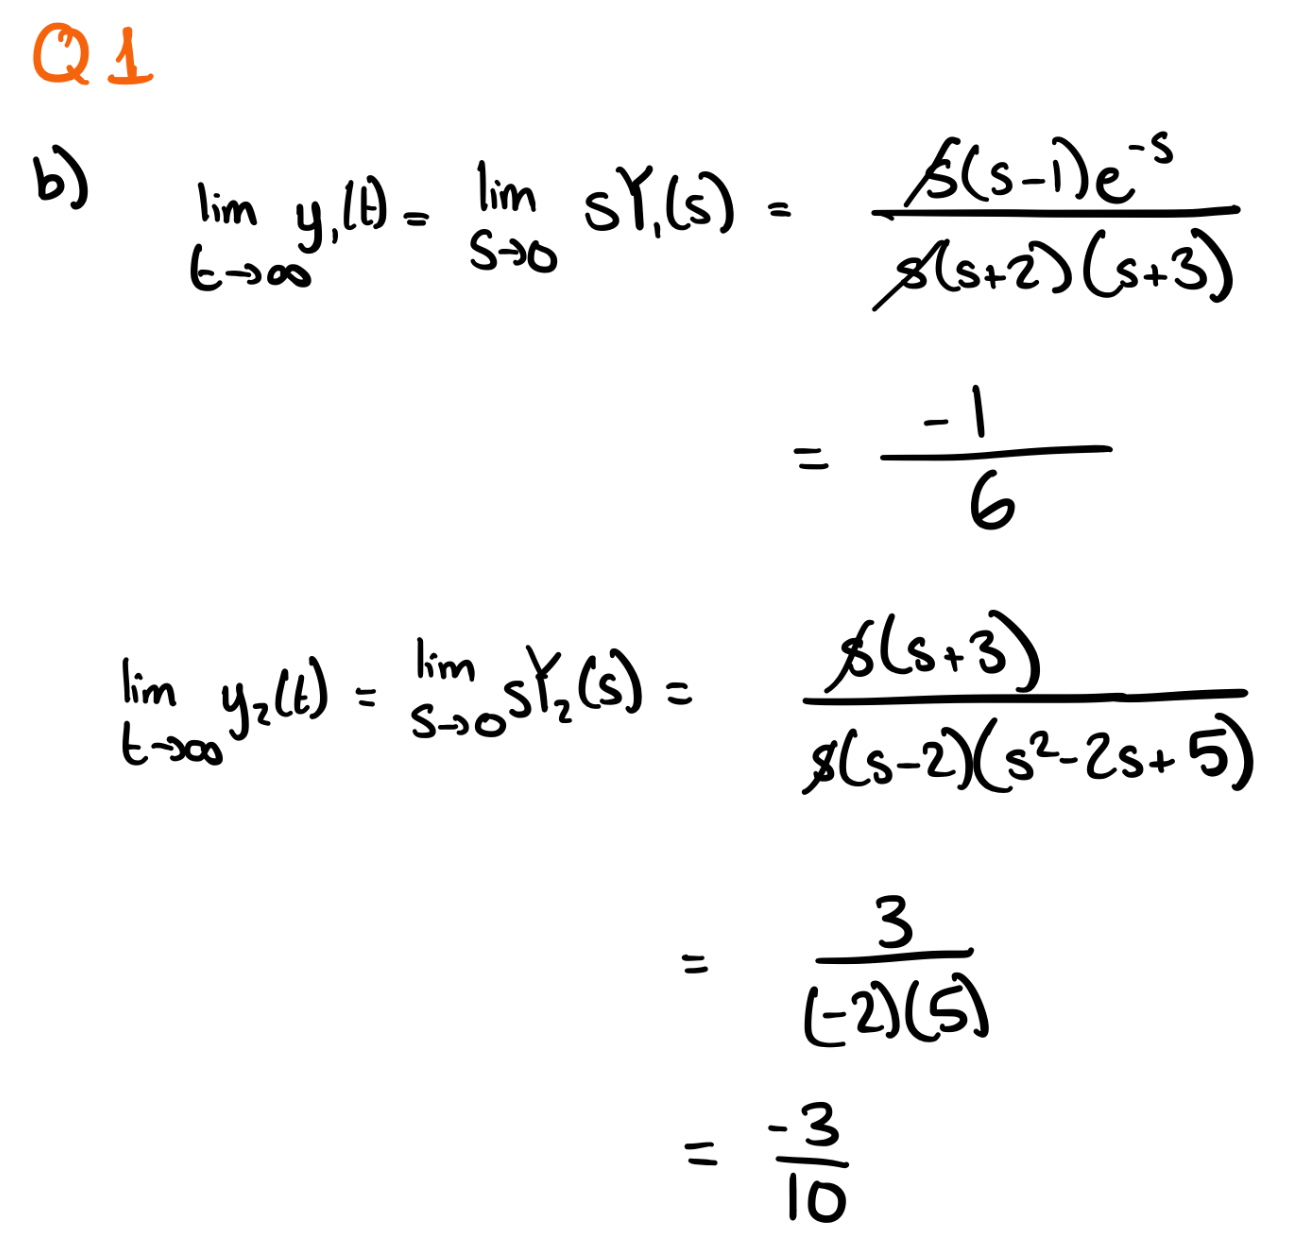
\includegraphics[width=0.6\textwidth]{Figures/handcalc/q1b.png}
      \caption{Final Value Theorem for \( Y_1(s) \) and \( Y_2(s) \)}
      \label{fig:figure14} 
    \end{figure}

    The calculations confirm that \( Y_1(s) \) settles to a finite negative value, whereas \( Y_2(s) \), despite being unstable in impulse response, has a well-defined steady-state when analyzed using Final Value Theorem.

    % ANSWER TO 1.3
    \item
    The impulse response for both systems was computed to observe the effect of the pole locations.

    - The response of \( Y_1(s) \) looks to be bounded confirming stability. \\
    - The response of \( Y_2(s) \) grows exponentially, which aligns with its unstable pole.

    \begin{figure}[H]
      \centering
      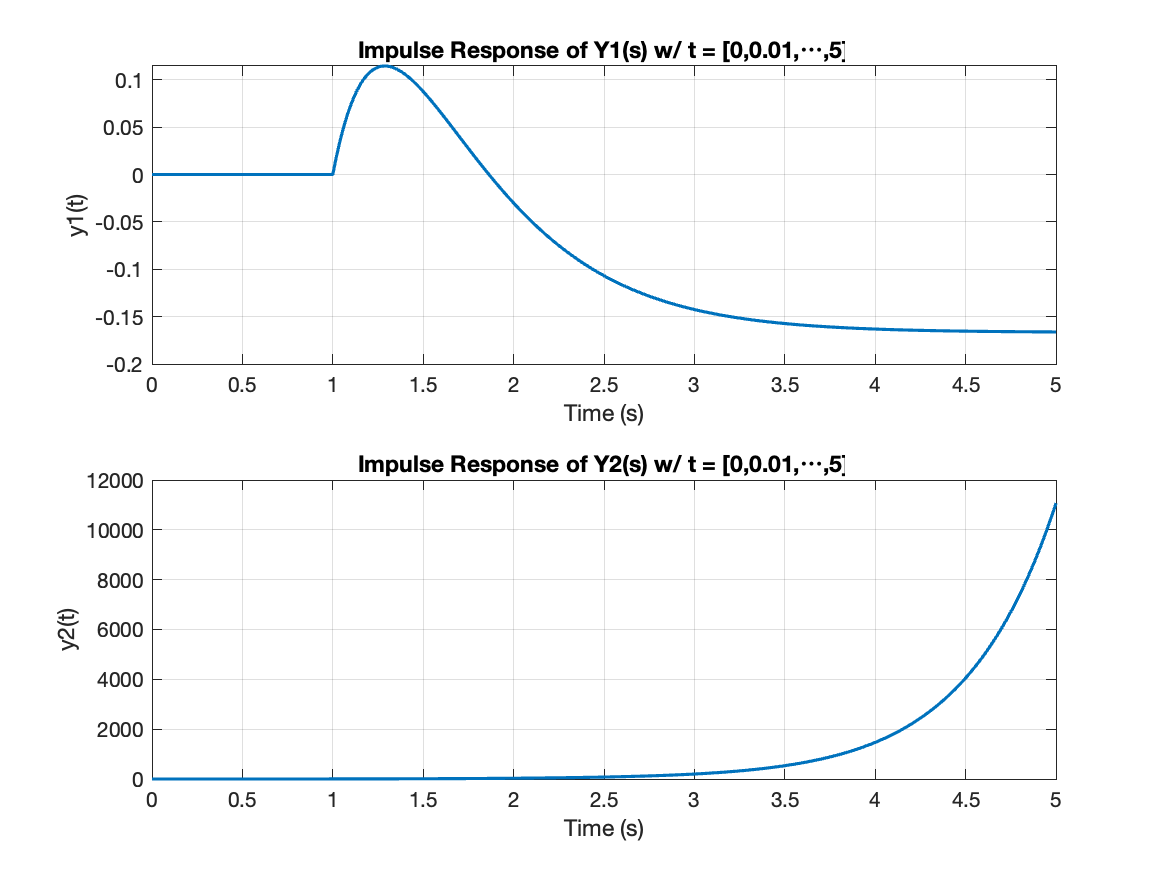
\includegraphics[width=0.9\textwidth]{Figures/figure1-3a.png}
      \caption{Impulse Response of \( Y_1(s) \) and \( Y_2(s) \) for \( t \in [0,5] \)}
      \label{fig:figure12} 
    \end{figure}

    Extending the time range further highlights the unstable growth of \( Y_2(s) \). Not only that, if you zoom into \( Y_1(s) \), you can see that the curve looks a little patchy since the time steps aren't small enough:

    \begin{figure}[H]
      \centering
      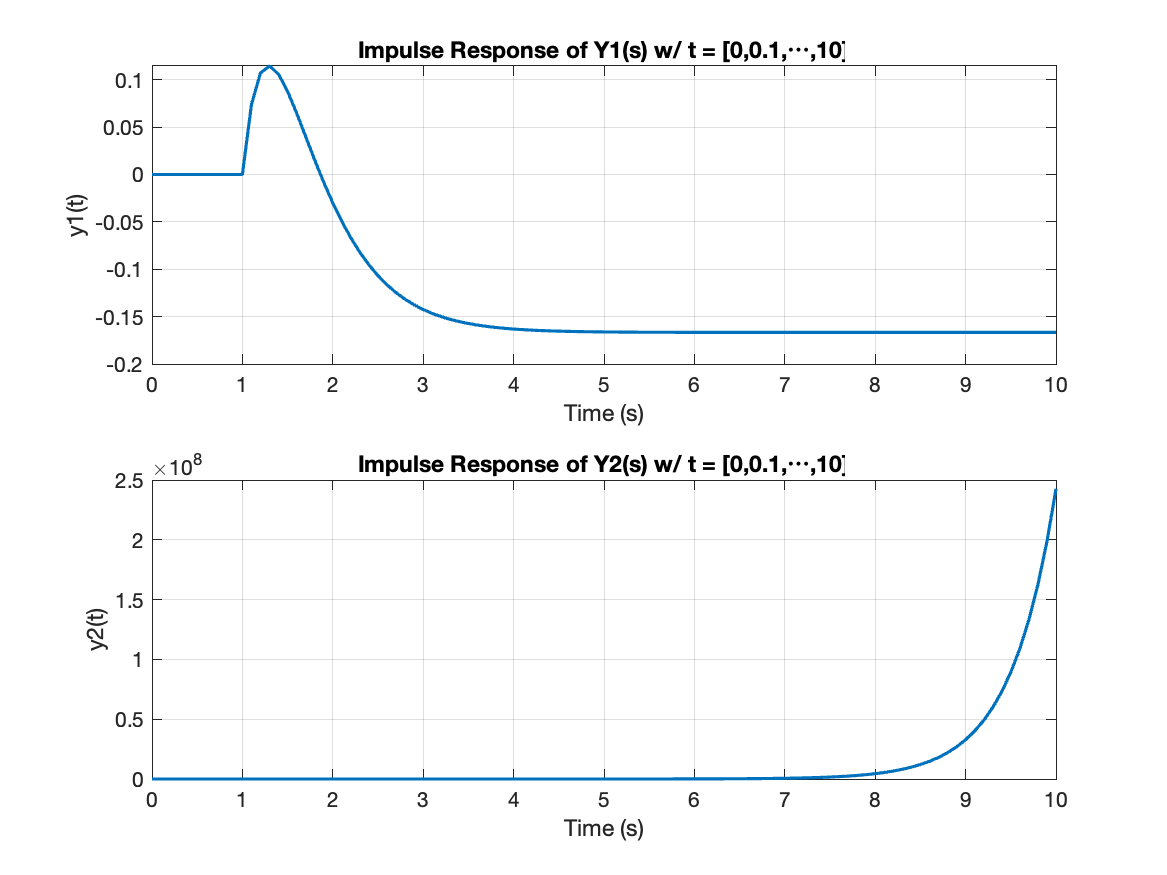
\includegraphics[width=0.9\textwidth]{Figures/figure1-3b.png}
      \caption{Impulse Response of \( Y_1(s) \) and \( Y_2(s) \) for \( t \in [0,10] \)}
      \label{fig:figure13} 
    \end{figure}

  \end{enumerate}

\pagebreak

\item Question 2
  \begin{enumerate}
    % ANSWER TO 2.1
    \item
    Below we've derived the transfer function model that relates the change in temperature of the thermocoupled $T$ to a change in the furnace temperature $T_F$.

    \begin{figure}[H]
      \centering
      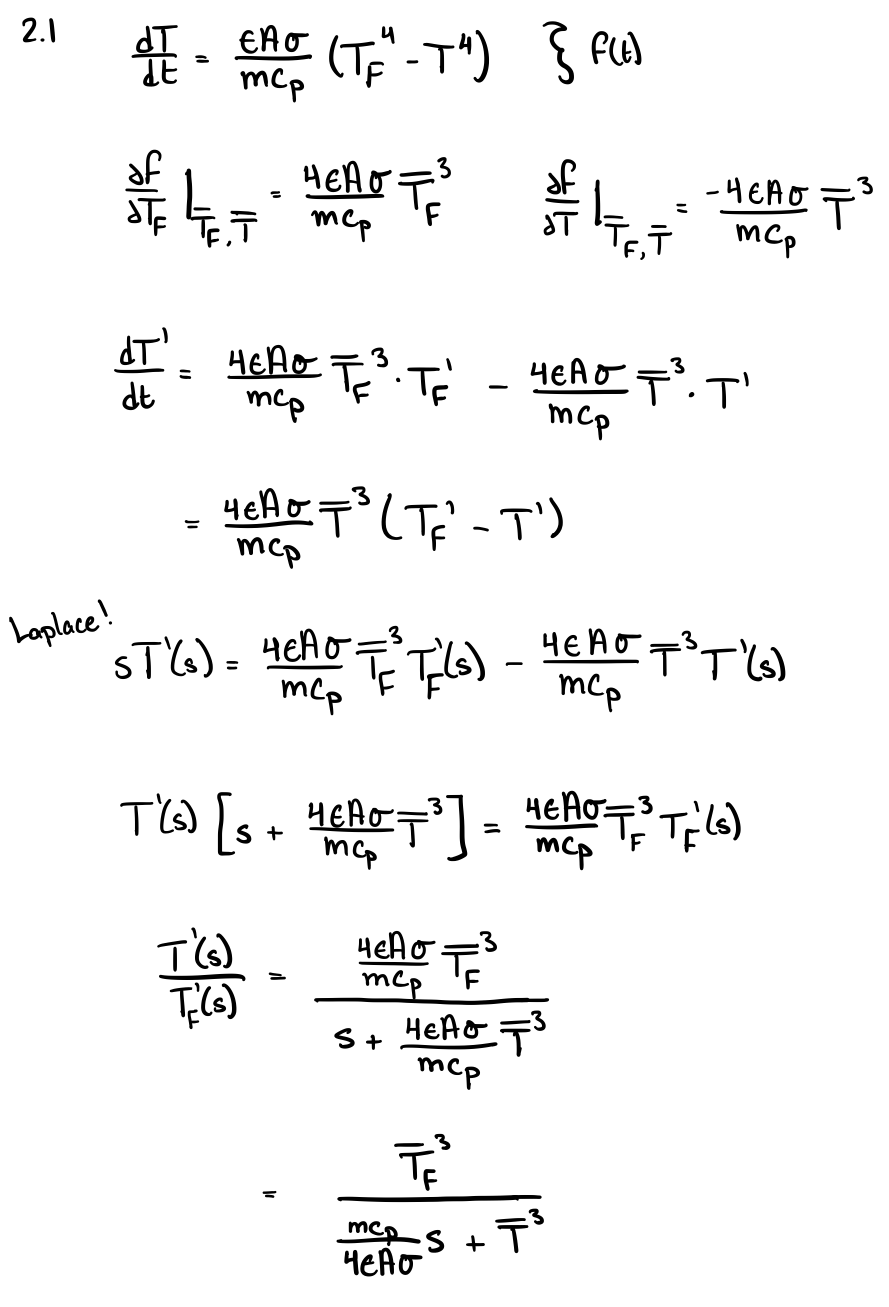
\includegraphics[width=0.6\textwidth]{Figures/handcalc/q2-1.png}
      \caption{Hand calculation to find $T'(s)/T_F'(s)$}
      \label{fig:figure21} 
    \end{figure}

  
    % ANSWER TO 2.2
    \item
    The thermocouple's response to a 30°C drop in furnace temperature was simulated using the linearized transfer function. 
    The step response of the thermocouple shows a gradual decrease in temperature, confirming that the thermocouple lags behind furnace temperature changes.

    \begin{figure}[H]
      \centering
      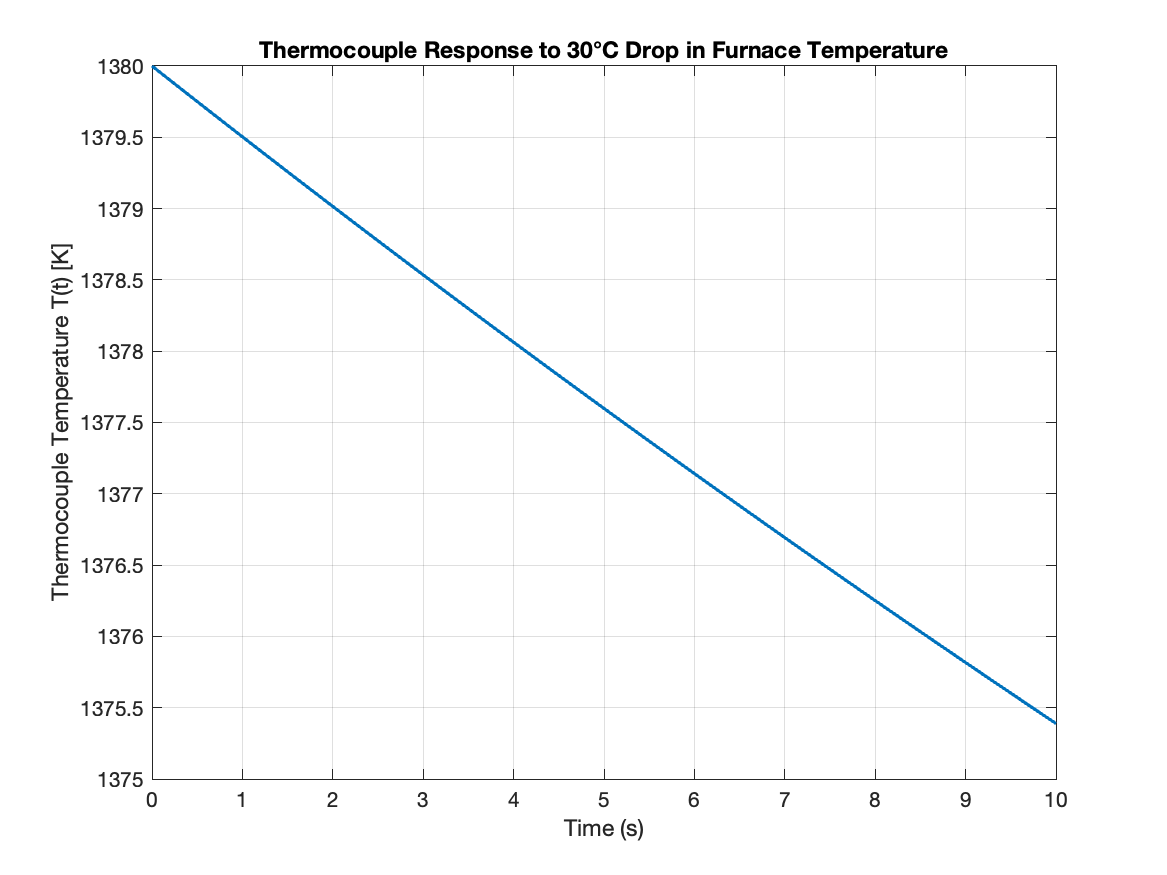
\includegraphics[width=1\textwidth]{Figures/figure2-2.png}
      \caption{Thermocouple Response to 30°C Drop in Furnace Temperature}
      \label{fig:figure22} 
    \end{figure}

    % ANSWER TO 2.3
    \item
    The nonlinear ODE model for the thermocouple temperature was simulated using ode45(). The resulting response follows a slightly curved trajectory, showing a more gradual cooling effect compared to the linearized model. You can see here, that it is relatively rapid towards the start and then slows down as time goes on.

    \begin{figure}[H]
      \centering
      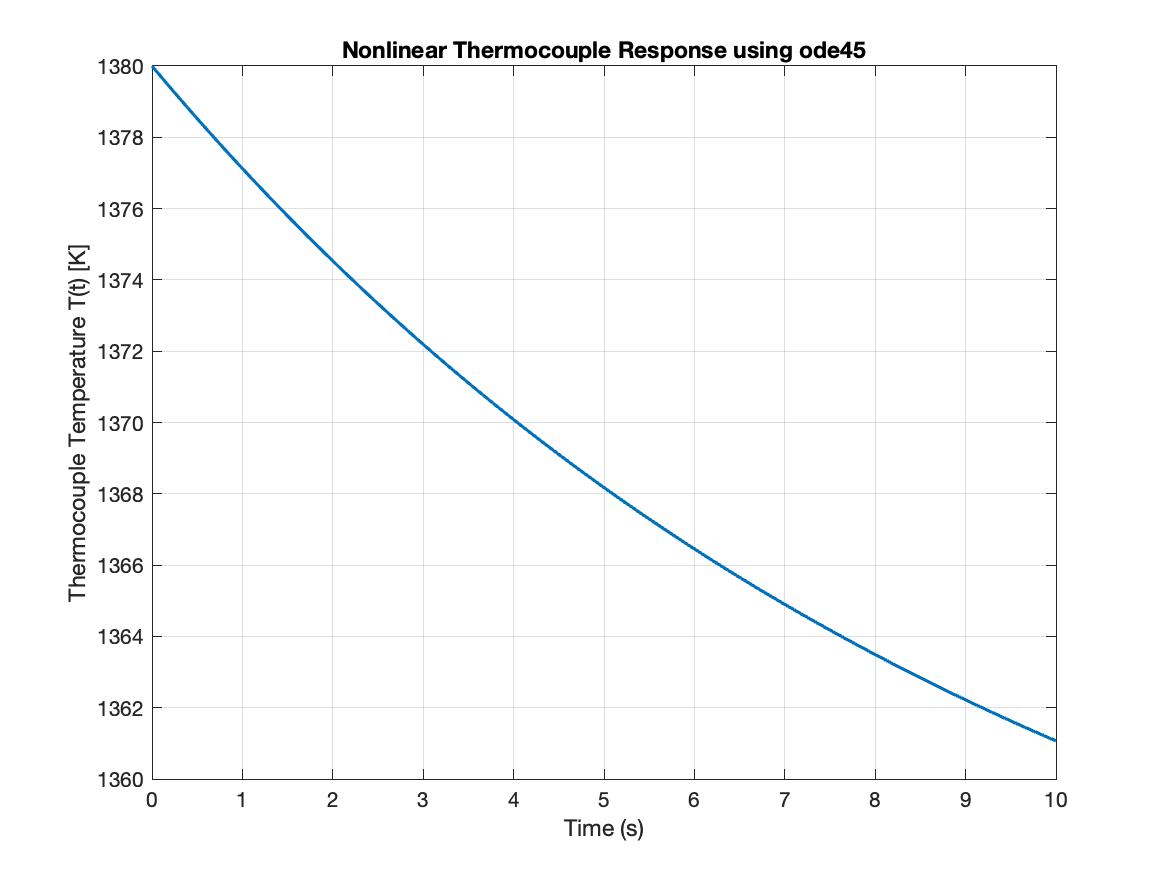
\includegraphics[width=1\textwidth]{Figures/figure2-3.png}
      \caption{Nonlinear Thermocouple Response using ode45}
      \label{fig:figure23} 
    \end{figure}

    % ANSWER TO 2.4
    \item
    A comparison of the linear and nonlinear models shows that the linearized transfer function underestimates the cooling rate. The nonlinear model predicts a faster response because radiative heat transfer follows the Stefan-Boltzmann Law, which is temperature-dependent and nonlinear. This means the rate of heat loss changes more significantly at higher temperatures compared to a simple linear approximation.

    \begin{figure}[H]
      \centering
      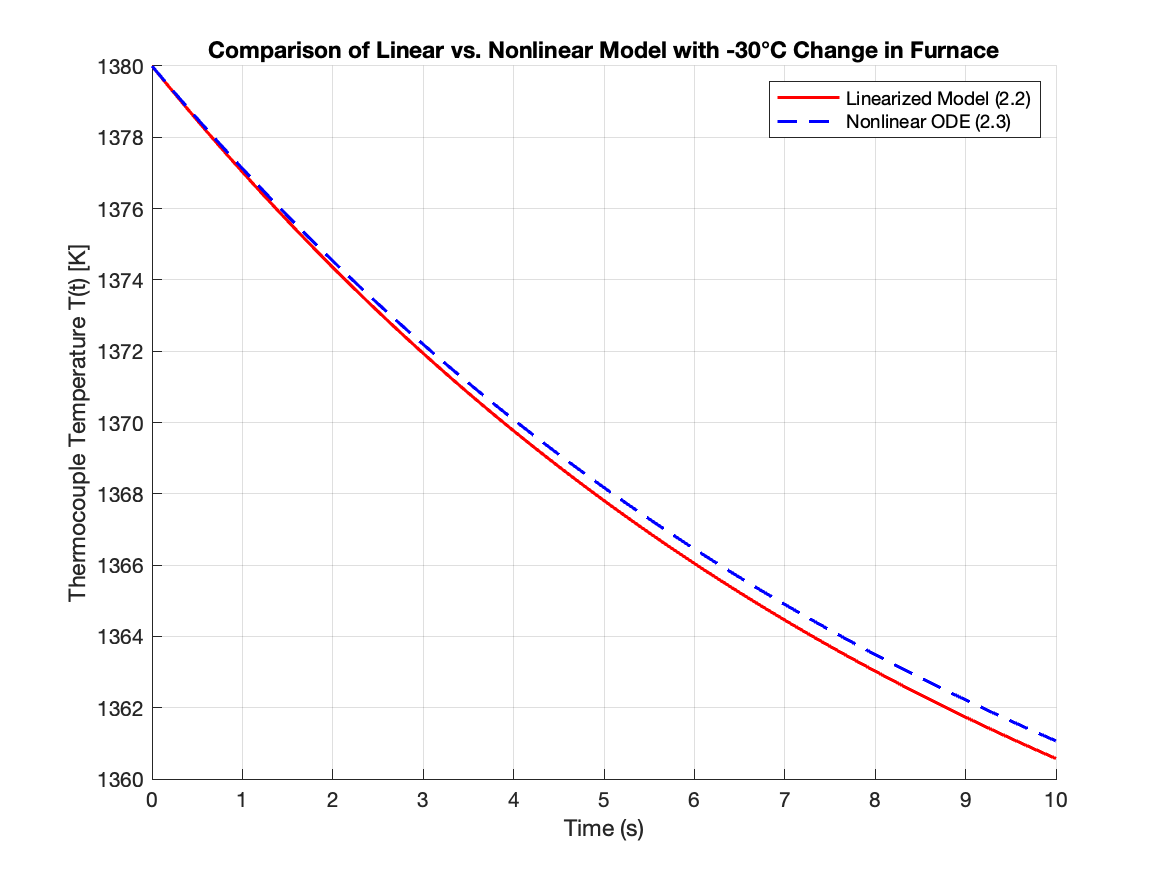
\includegraphics[width=1\textwidth]{Figures/figure2-4a.png}
      \caption{Comparison of Linear vs. Nonlinear Model with +30°C Change in Furnace}
      \label{fig:figure24a} 
    \end{figure}

    \begin{figure}[H]
      \centering
      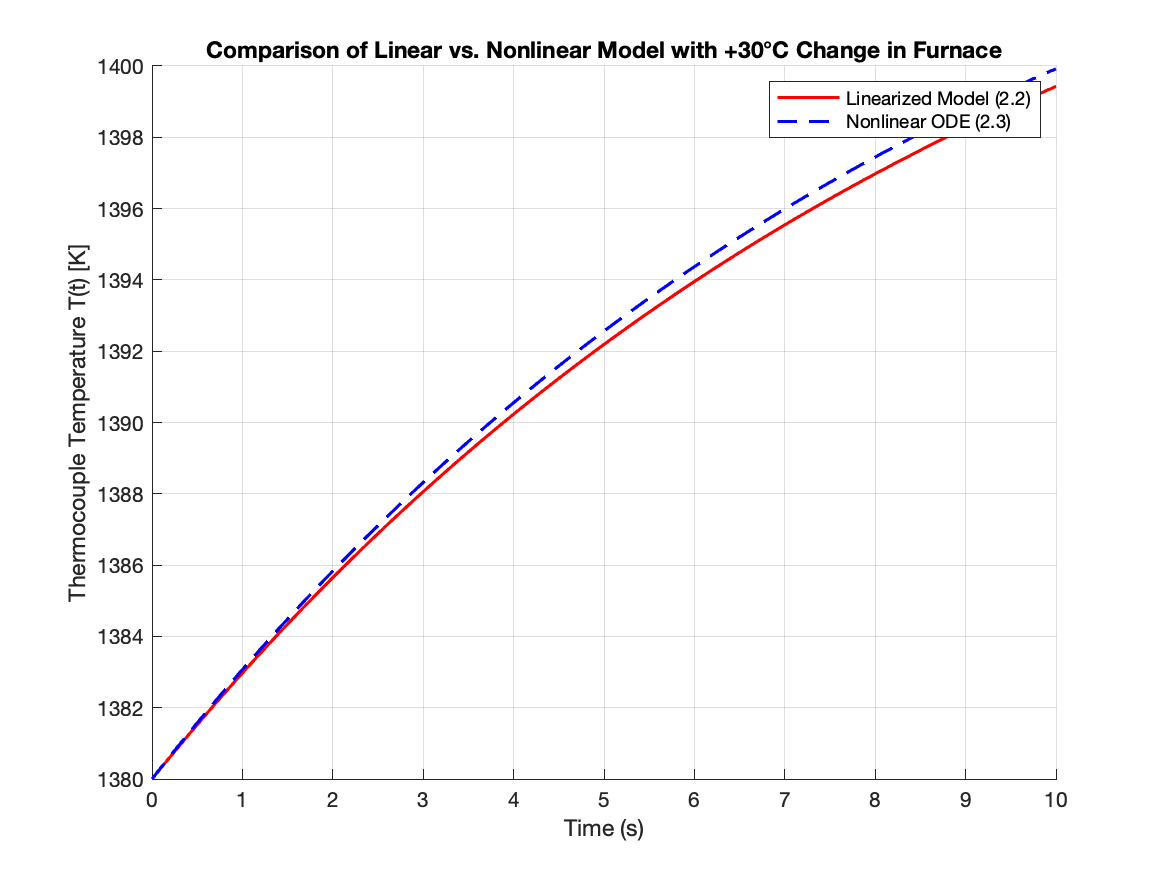
\includegraphics[width=1\textwidth]{Figures/figure2-4b.png}
      \caption{Comparison of Linear vs. Nonlinear Model with -30°C Change in Furnace}
      \label{fig:figure24b} 
    \end{figure}

    % ANSWER TO 2.5
    \item
    In this case, we analyzed the effect of heat input \( Q(t) \) on the thermocouple temperature. The furnace response to \( Q(t) \) was modeled, and the thermocouple's response was calculated by multiplying the transfer functions:

    \[
    \frac{T(s)}{Q(s)} = \frac{T(s)}{T_F(s)} \times \frac{T_F(s)}{Q(s)}
    \]

    \begin{figure}[H]
      \centering
      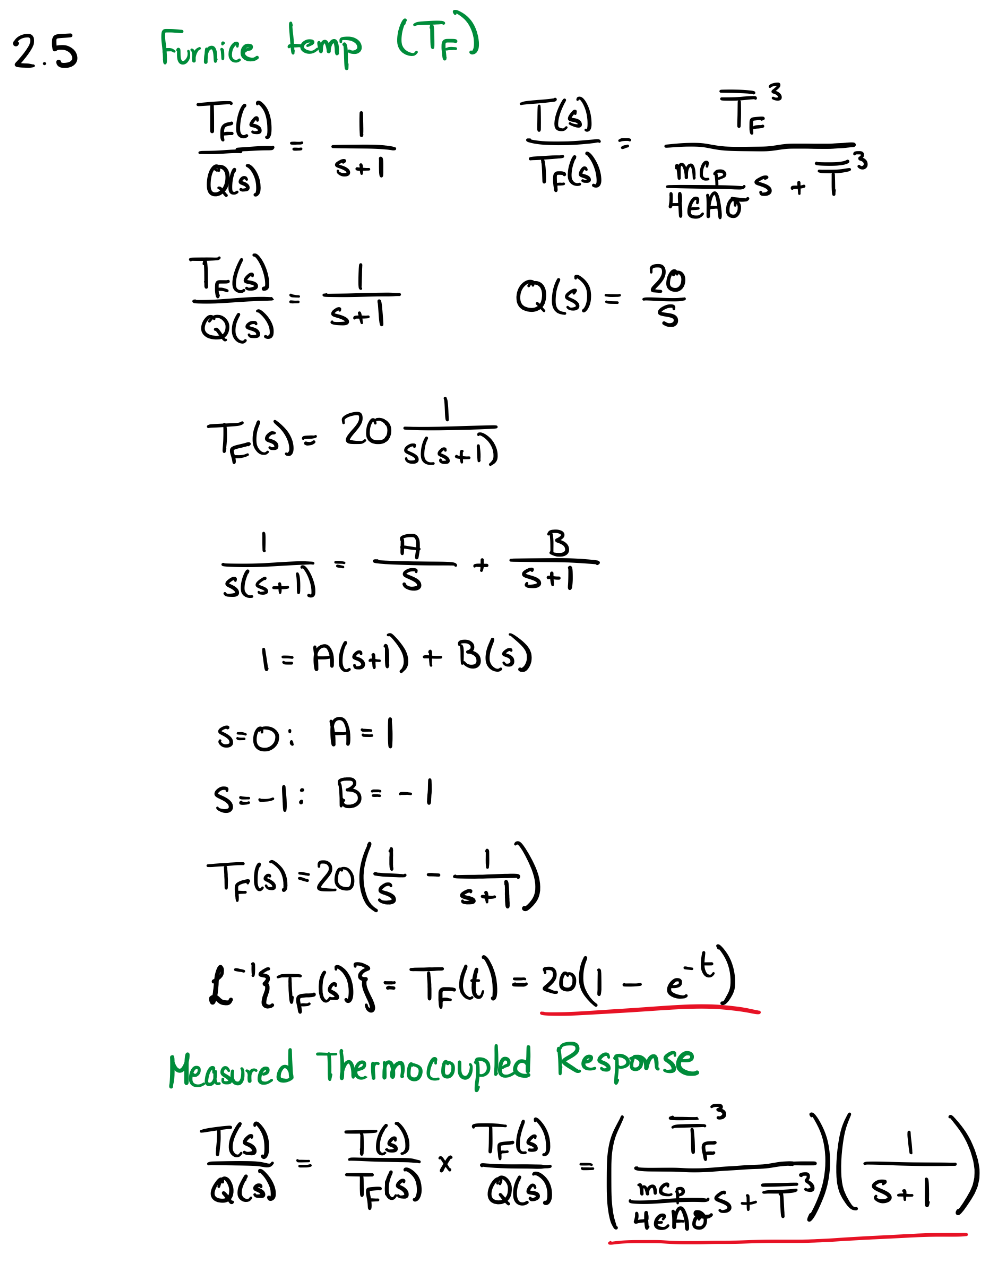
\includegraphics[width=0.7\textwidth]{Figures/handcalc/q2-5.png}
      \caption{Hand calculation to find $T_F(s)$ and $T(s)$ given the new $Q(s)$ input.}
      \label{fig:figure25a} 
    \end{figure}

    The final response shows a delayed and gradual increase in temperature, confirming that both the furnace and thermocouple introduce time lag in heat transfer.

    The final response shows a delayed and gradual increase in temperature, confirming that both the furnace and thermocouple introduce time lag in heat transfer. Notably, \( T_F(t) \) responds much faster to the step change in heat input, reaching its new steady-state value quickly. In contrast, \( T(t) \) (thermocouple reading) lags significantly, indicating that the thermocouple has a much slower thermal response. Knowing about this delay is critical in control applications, as for example, in this case, it means that relying solely on the thermocouple reading for feedback could lead to incorrect adjustments due to outdated temperature measurements.

    \begin{figure}[H]
      \centering
      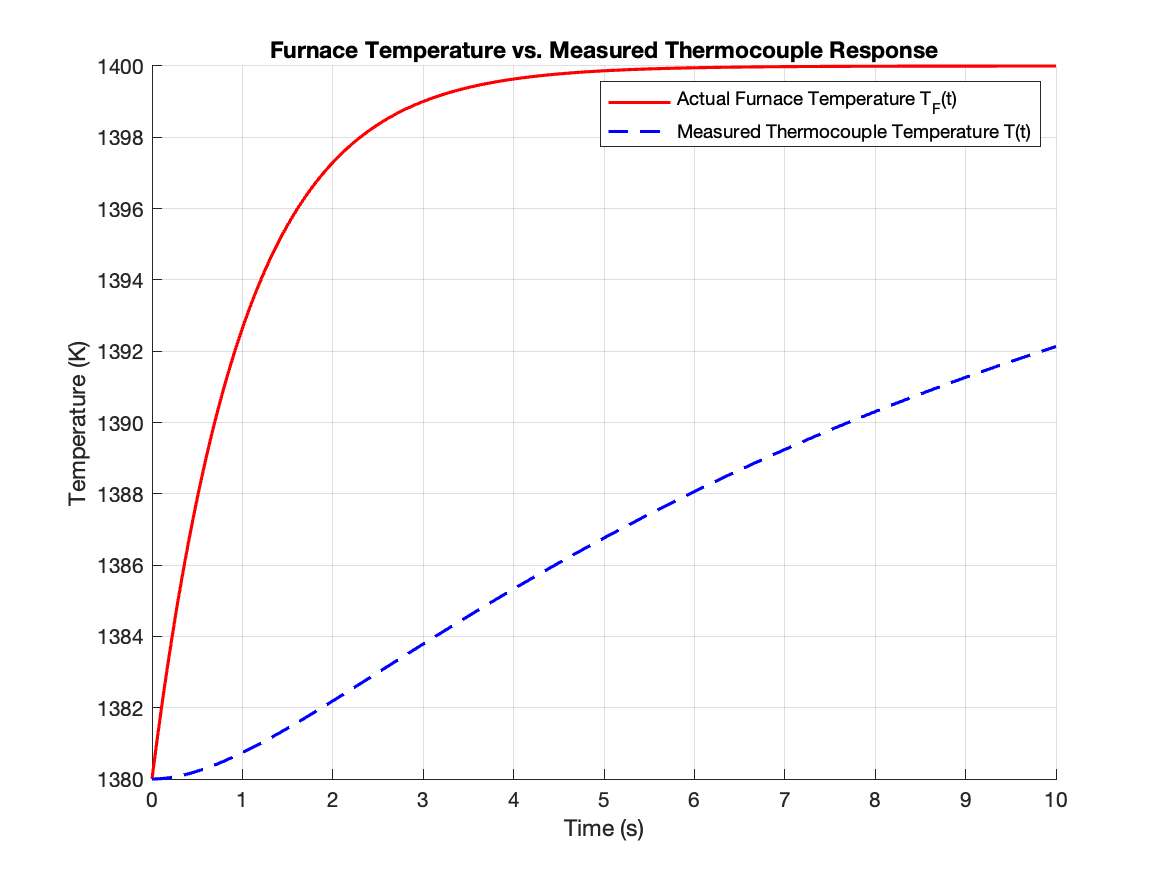
\includegraphics[width=1\textwidth]{Figures/figure2-5.png}
      \caption{Furnace Temperature vs. Measured Thermocouple Response with Heat Input \( Q \)}
      \label{fig:figure25b}
    \end{figure}

  \end{enumerate}

\end{enumerate}

\end{document}
